\section{Алгоритм генерации сцены}

Для генерации сцены будет использован алгоритм квантового коллапса волновой функции. 

Для корректной работы алгоритма крайне важно правильное задание начальных ограничений. Под ограничением подразумевается возможность или невозможность появления определённой ячейки вплотную к другой ячейке с определённой стороны~\cite{QWFC}.

Например, если в одной ячейке содержится прямой участок дороги, то к тем сторонам ячейки, которые пересекает дорога, могут быть "присоединены" только такие ячейки, в которых к этим же сторонам будут присоединены другие участки дороги. Это ограничение изображено на рисунке~\ref{fig:restrictions}.

\begin{figure}[h!]
    \centering
    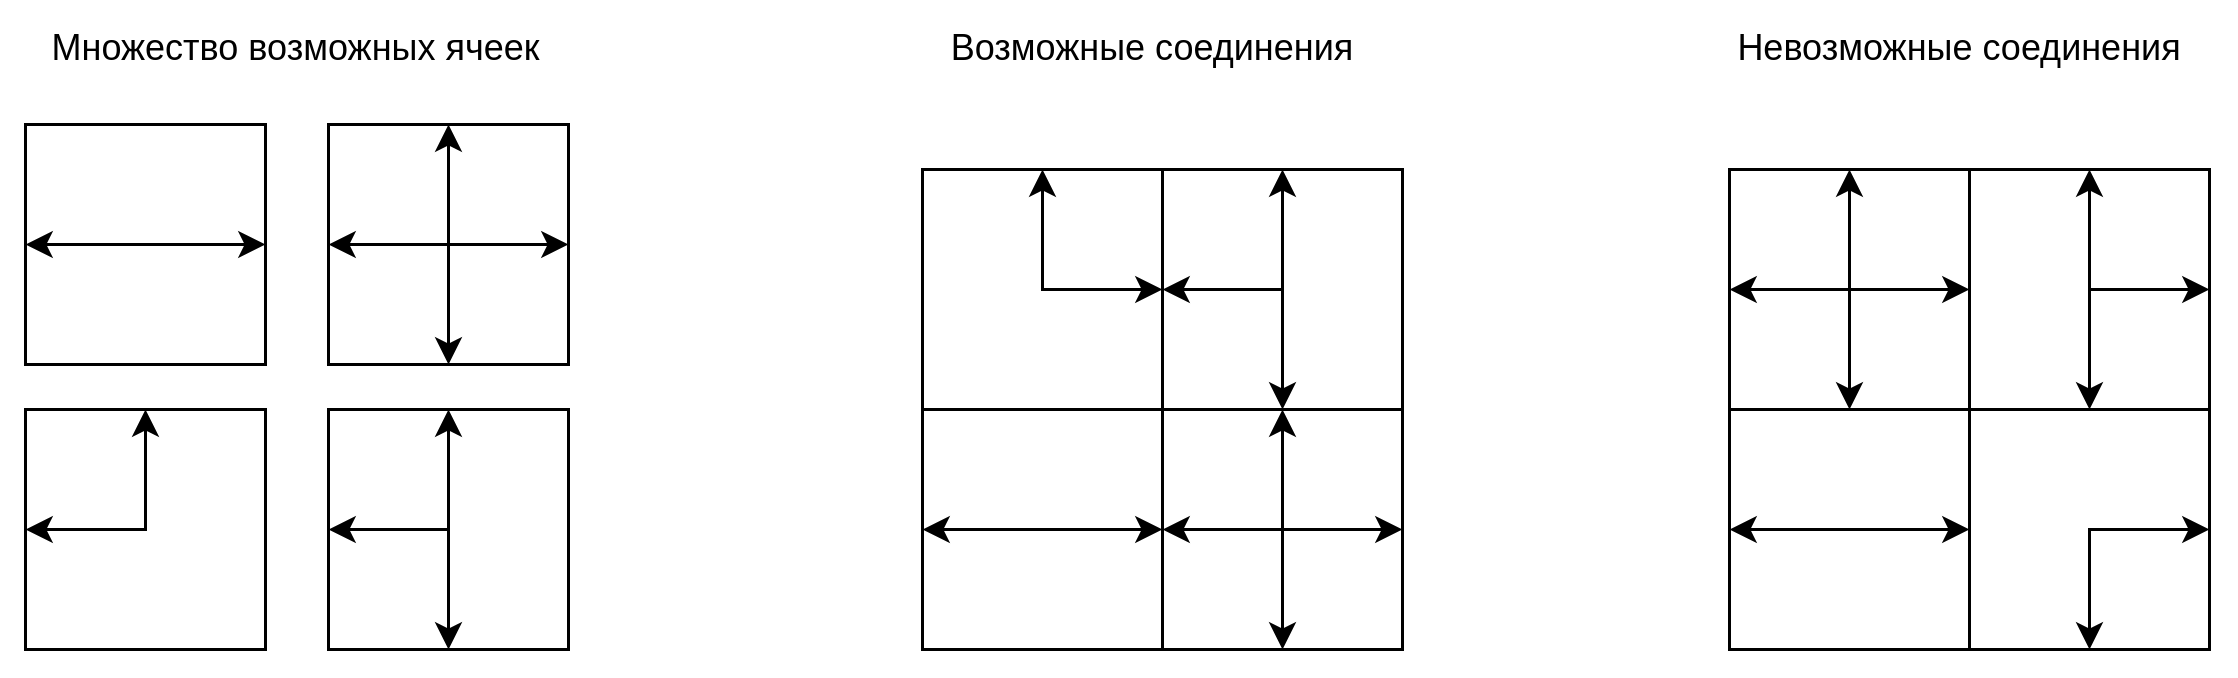
\includegraphics[width=.9\textwidth]{restrictions.drawio.png}
    \caption{Визуализация ограничений генерации}
    \label{fig:restrictions}
\end{figure}

Описание ограничений выполняется вручную для каждой возможной ячейки и её поворота, однако этот процесс можно значительно упростить, если учитывать симметрию и возможные повороты ячеек на уровне программного кода. 

Пусть необходимо заполнить матрицу генерации $M$ размеров 50 на 50 ячеек. Изначально все ячейки находятся в состоянии суперпозиции, то есть каждая ячейка может принять любое возможное значение. Возможные значения, в свою очередь, определяются пересечением ограничений соседних ячеек. Если какой-либо из соседей не находится в строго определённом состоянии, его ограничениями будет являться объединение ограничений каждого из возможных состояний.

Пока все ячейки матрицы не примут строго определённое состояние, выполняется цикл, который выбирает ячейку с наименьшим количеством возможных состояний и фиксирует её значение, случайным образом выбирая одно из возможных значений.

Предусмотрена возможность повлиять на вероятность выбора того или иного состояния ячейки путём задания ему некоторого веса. Например, для случая с дорогами, можно повысить вероятность появления поворота и уменьшить вероятность появления перекрёстка.

После обновления ячейки в матрице, ограничения её соседей обновляются.

Алгоритм коллапса волновой функции представлен на рисунке~\ref{fig:QWFC}

\newpage

\begin{figure}[h!]
    \centering
    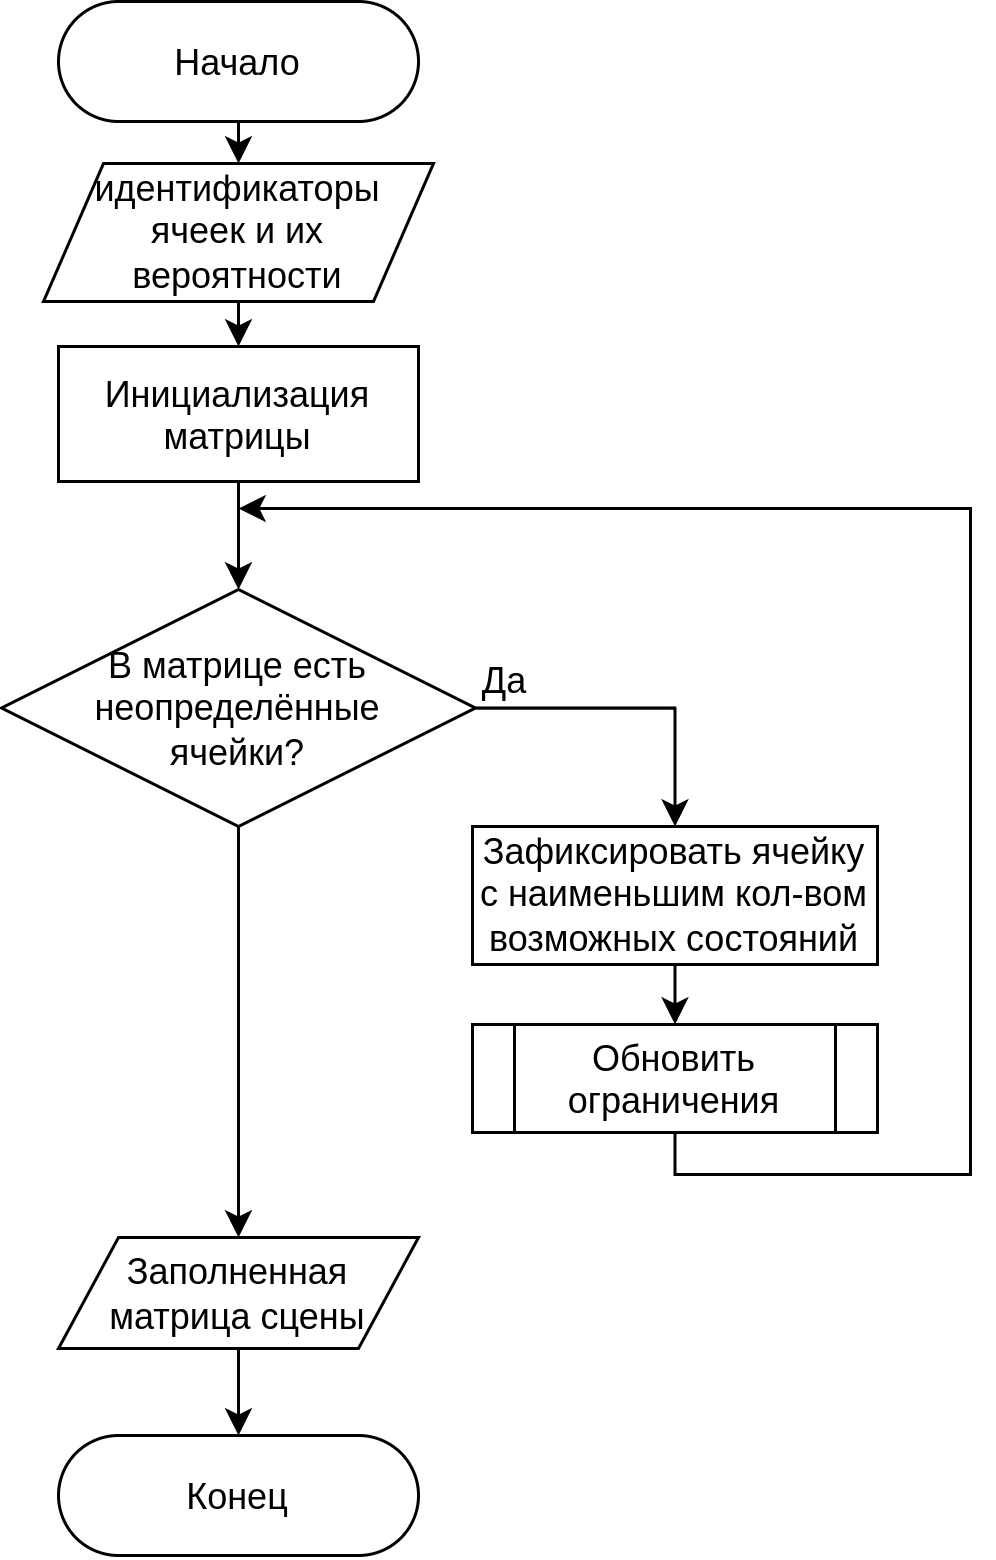
\includegraphics[width=.8\textwidth]{QWFC.drawio.png}
    \caption{Алгоритм квантового коллапса волновой функции}
    \label{fig:QWFC}
\end{figure}

В рамках данной работы будут использованы 10 типов ячеек:

\begin{itemize}
    \item дорожный перекрёсток;
    \item горизонтальный прямой участок дороги;
    \item вертикальный прямой участок дороги;
    \item 4 типа угловых участков дороги;
    \item пустырь;
    \item дерево;
    \item дом.
\end{itemize}

Поскольку ячеек для описания разных типов дорог семь, а остальных ячеек всего три, необходимо снизить вероятность появления каждого определённого типа дороги в семь раз. Такое снижение вероятности сравняло бы шансы появления дороги или другого типа объекта в той или иной ячейке матрицы, однако вероятности дорог снижены неравномерно для уменьшения количества перекрёстков и поворотов.

Таким образом, получаем скорректированные вероятности появления:
\begin{itemize}
    \item перекрёстка --- 10\%;
    \item прямых участков --- 25\%;
    \item угловых участков --- 10\%;
\end{itemize}

Соотношение других типов объектов (и дорог) друг к другу также можно будет корректировать в интерфейсе приложения.
